\documentclass[conference]{IEEEtran}




\usepackage{amssymb}
\usepackage{amsmath}
\usepackage{graphicx}
%\usepackage{lipsum}
\usepackage{verbatim}

\usepackage{multirow}
\usepackage{color}
\usepackage{colortbl}
\usepackage{ifpdf}
\usepackage{url}
\usepackage[bookmarks=false]{hyperref}
\usepackage{hhline}
\usepackage[printonlyused]{acronym}
%\usepackage{appendix}
\usepackage{breakurl}
%\usepackage[style=super]{glossaries}
\usepackage{longtable}
\usepackage{enumerate}
%\usepackage{tikz}
%\usepackage{rotating}
\usepackage{lineno}
%\usepackage{graphics}
\usepackage[table]{xcolor}
\usepackage{threeparttable}
\usepackage{algorithm}
\usepackage{setspace}

\newcommand\BibTeX{{\rmfamily B\kern-.05em \textsc{i\kern-.025em b}\kern-.08em
T\kern-.1667em\lower.7ex\hbox{E}\kern-.125emX}}


\DeclareGraphicsExtensions{.pdf,.png,.jpg}
\graphicspath{{images/}}

% Put remarks in the paper easily located by ``bigodot'' in margin
% Usage: \todo{twf: we need a better example here.}
\newcommand{\todo}[1]{%
\mbox{}\marginpar[\hfill$\bigodot$]{$\bigodot$\hfill}
{\bf \sc #1}}



\acrodef{RBAC}{Role Based Access Control}
\acrodef{EMS}{Electronic Marking System}


\definecolor{lightblue}{rgb}{0.93,0.95,1.0}
\definecolor{babyblueeyes}{rgb}{0.63, 0.79, 0.95}


\begin{document}



\title{Incremental Development of RBAC-controlled E-marking System Using the B Method}

{\author{\IEEEauthorblockN{Nasser Al-Hadhrami
\IEEEauthorblockA{School of Computing\\
University of Portsmouth,
UK\\
}}
\and
\IEEEauthorblockN{Benjamin Aziz
\IEEEauthorblockA{School of Computing\\
University of Portsmouth,
UK\\
}
\and
\IEEEauthorblockN{Shantanu Sardesai}
\IEEEauthorblockN{Technical University of \\ 
Darmstadt, Germany\\
}}
\and
\IEEEauthorblockN{Lotfi ben Othmane}
\IEEEauthorblockA{
Fraunhofer SIT\\
Germany\\}
}

\maketitle

\begin{abstract}

\ac{RBAC} models are access policies that associate access rights to roles of subjects on objects. The incremental development of software by adding new features and the insertion of new access rules potentially render the model inconsistent and create security flaws. This paper proposes modeling \ac{RBAC} models using the B language such that it is possible to reevaluate the consistency of the models following model changes. It shows the mechanism of formalizing \ac{RBAC} policies of an \ac{EMS} using B specifications and illustrates the verification of the consistency of the \ac{RBAC} specification, using model checking and proof obligations.

\end{abstract}

\begin{IEEEkeywords}
Role Based Access Control (RBAC), formal specifications, RBAC constraints, separation of duties, role hierarchy, cardinality constraints, model checking, proof obligations.
\end{IEEEkeywords}
\acresetall

% general terms are not compulsory anymore, 
% you may leave them out

%\keywords
%\Keyword: Software Security; agile software security; systematic review study
 
\maketitle




\section{Introduction} 

Security is now becoming a very important aspect when it comes to the development of modern systems. Many critical systems, especially those which handle commercial transactions, enforce different security policies to their systems in order to ensure that existing data and information flow are secure enough to preserve confidentiality. If there is any defect in applying any security policy to a particular system, as if specifying ambiguous properties or defining inconsistent model, then the system might lack reliability. Hence, formal methods are widely used to verify the correctness and consistency of most of security models, including \ac{RBAC} policies, as they rely on \textit{mathematical logic} and \textit{set theory}~\cite{DBS2004}.

RBAC model is regarded as a successful alternative to discretionary and mandatory access control models.  Efficiently, \ac{RBAC} can be more suitable for commercial systems, since it depends essentially on assigning different users to particular roles~\cite{FeKu2009}. However, \ac{RBAC} policy is not restricted to business systems only, but also to any critical system that needs to determine whether a given subject (user) is allowed to access a certain object (resource). 
This paper discusses a study case: \ac{EMS} in Oman Secondary Schools, where \ac{RBAC} security policy needs to be applied to.  EMS aims at providing a consolidated environment, where each member within a school has the right to access the system within the powers (authorizations) given to him/her. For example, teachers can access the system for the purpose of adding, editing or deleting marks.  Whereas, students have the authorization to submit reports and view their grades.



\subsection{The B Refinement Method}

The B method \cite{Abrial-BBook-1996} is a formal method for specifying, refining and implementing software.  B is a refinement methodology as it allows the system developer to start with an abstract model of the system considering its context, and gradually add details to the model leading to a sequence of more concrete models until the final implementation is reached.  The model development process creates a number of \textit{proof obligations}, which guarantee the correctness of the model as well as any desired invariants (properties) that the model of the system should preserve. Proof obligations can then be proven by automatic or interactive theorem provers or model checking tools, and the model itself can be simulated in runtime.  The proving of obligations as well as checking invariants and simulating the model are functions that are well supported by tools such as \textit{ProB} \cite{LeuschelB03}.

For the rest of the paper, we do not use the refinement part of B, and we constrain ourselves to the use of B as a formal language to specify one mode of the RBAC policies for the case of e-marking systems.   Therefore, we revisit the formalisation of the desirable properties in the system in Section \ref{sec:verification}.



\section{RBAC Security Policy}\label{sec:background} 

RBAC is one of the most efficient models of access control policies~\cite{AhHu2007}.  Began in 1970s with multi-user and multi-application, and has rapidly evolved in the last three decades as a technology for applying a high level security in large-scale systems.  The pivotal idea behind RBAC model is that permissions are associated with roles, and users are administratively assigned to proper roles~\cite{Zha2008}. This mechanism ensures that only authorized users can perform some functions on some data/resources~\cite{FeKu2009}. Generally, RBAC model consists of some basic elements, such as Users, Roles, Permissions, User Assignment (UA), Permissions Assignment (PA) and Constraints (see Figure 1).

\begin{figure}[bht]
\centering
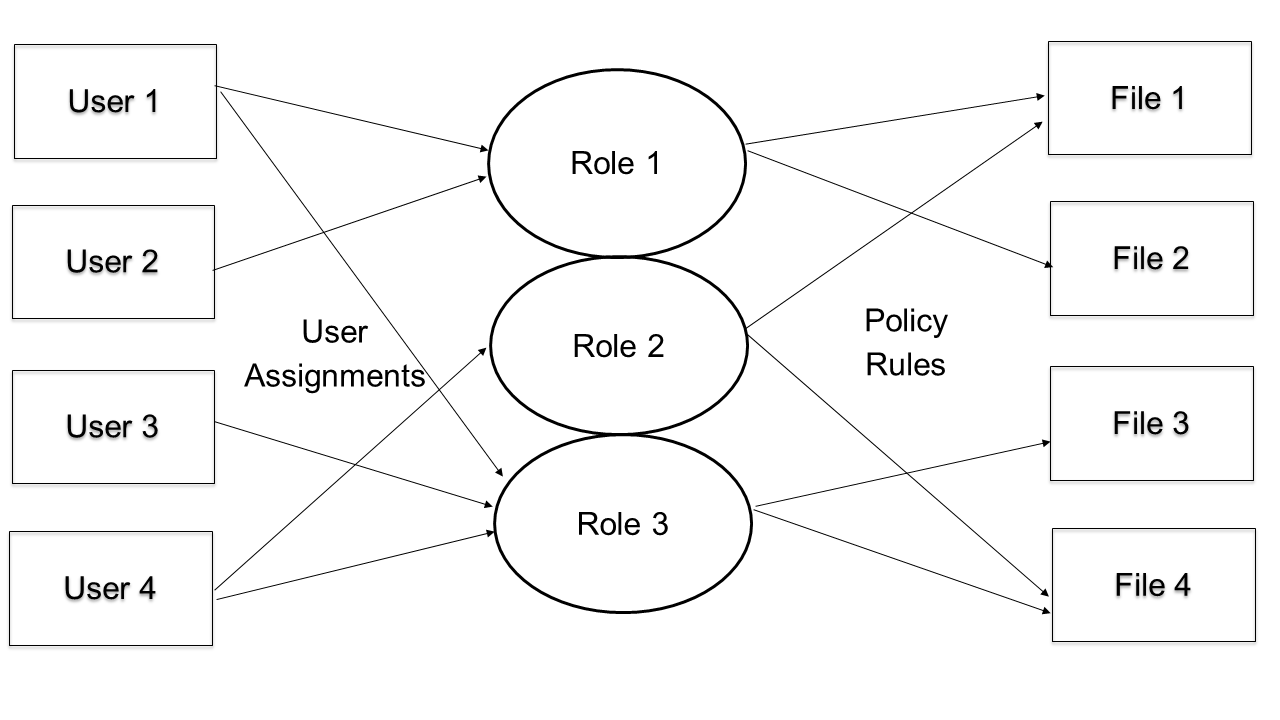
\includegraphics[scale=0.26]{RBACpolicy.png}
\caption{The concept of RBAC security policy.}
\label{fig:RBACPol}
\end{figure}


It is clear that users are not mapped directly into permissions of accessing some resources, but to specific roles which have to be previously assigned to those permissions~\cite{YuBr2012}.  For example, in medical systems, nurses are authorized to access specific resources (e.g. files) which certainly differ from those in which physicians are allowed to.  Therefore, each role in the system (i.e. nurse and physician) is being mapped into the corresponding permissions.  If Alice, for instance, is a nurse, then she has to be assigned to the role $nurse$~\cite{DBS2004}. 
      In RBAC model, there are some relevant terms and concepts, which define the different model's elements~\cite{SDAG2008} (see Figure 2).  However, not all of them are necessary to represent an RBAC security policy, where there are some models that describe only certain needs for a particular system.

\begin{figure}[bht]
\centering
\includegraphics[scale=0.25]{RBACelements.png}
\caption{Elements of RBAC security policy.}
\label{fig:elelmRBAC}
\end{figure}



Table \ref{tab:elements} provides descriptions for the different elements in RBAC models.

\begin{table*}[bth]
\centering
\caption{Description of RBAC's elements.}
\small
\rowcolors{0}{}{lightblue}
\begin{tabular}{p{1.6 in} p{5.2 in}} \hline 
\hline
Code & Description\\\hline

Users (U)&  persons who interact with a system.\\
Roles (R)& prescribed behaviours, which describe particular positions or functions within an organization. \\
Permissions (P)& descriptions of the type of interactions that a user can have with an object.\\
Object& a passive entity that has some information, and   can receive new information.\\
User Assignment (UA)&a many-to-many relationship between users and roles.\\
Permission Assignment (PA)& a many-to-many relationship between permissions and roles.\\
Session (S)& a mapping between a user and any activated role/s that the user is assigned to.\\
Role Hierarchy (RH)& a partial order relationship on roles.\\
Constraints&restrictions on any of the above relationships/assignments.  \\ \hline\hline

\end{tabular}
\label{tab:elements}


\end{table*}




\section{RBAC Models}\label{sec:models} 

There is a family of four conceptual models for RBAC security policy, which define the various dimensions of it~\cite{PTN2009}. $RBAC_0$ is considered as the basic model, which has the minimum requirements for a system.  Whereas, $RBAC_1$, $RBAC_2$ and $RBAC_3$ are more advanced models.  However, the latter models are based on the basic one, $RBAC_0$, as some elements are common for all types of models~\cite{AhHu2007}.

$RBAC_0$ contains some basic elements of RBAC policies, that are required when defining any security policy for a system.  Usually, components of $RBAC_0$ are Users (U), Roles (R), Permissions (P), Sessions (S) as well as relationships between them. In addition to the components of $RBAC_0$, $RBAC_1$ model supports the concept of Role Hierarchy (RH).  Hierarchical of roles describe the gradualism of authorizations and responsibilities in an organization.  In other words, RH is about defining what is called senior roles (more powerful roles) and junior roles (less powerful roles), where senior roles may inherit permissions that are assigned to junior roles.

\begin{figure}[bht]
\centering
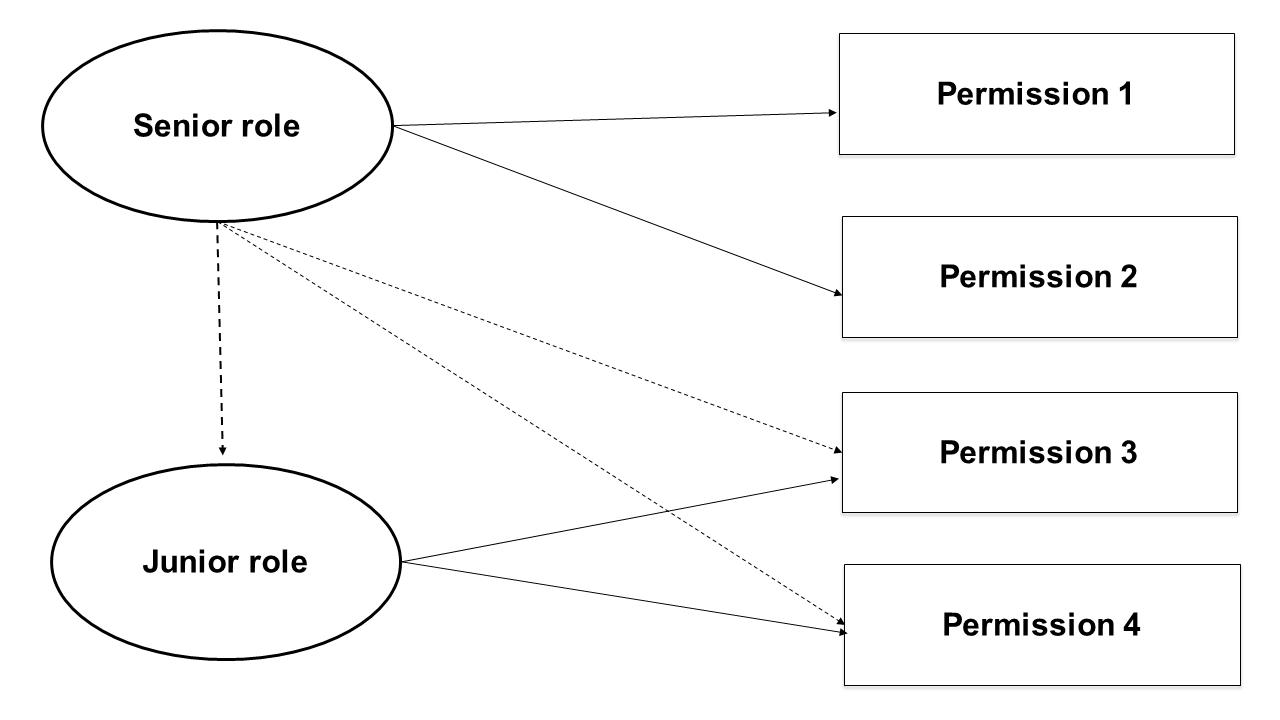
\includegraphics[scale=0.26]{RolesHierachy.png}
\caption{Role Hierarchy.}
\label{fig:RBACPol}
\end{figure}

In order to provide a powerful protection to the RBAC-based systems, $RBAC_2$ (constraints model) is defined to be the main driver of RBAC security policies.  That is $RBAC_2$ uses a mechanism to force restrictions and form a high level security policy.  Constraints can be applied to any relationship/assignment that has been defined in the two previous models, such as UA, PA, Sessions and Role Hierarchy (RH) (see Figure 4).  There are many types of applicable constraints, in particular those which deal with exclusiveness of roles (Separation of Duties) and cardinality constraints.


\begin{figure}[bht]
\centering
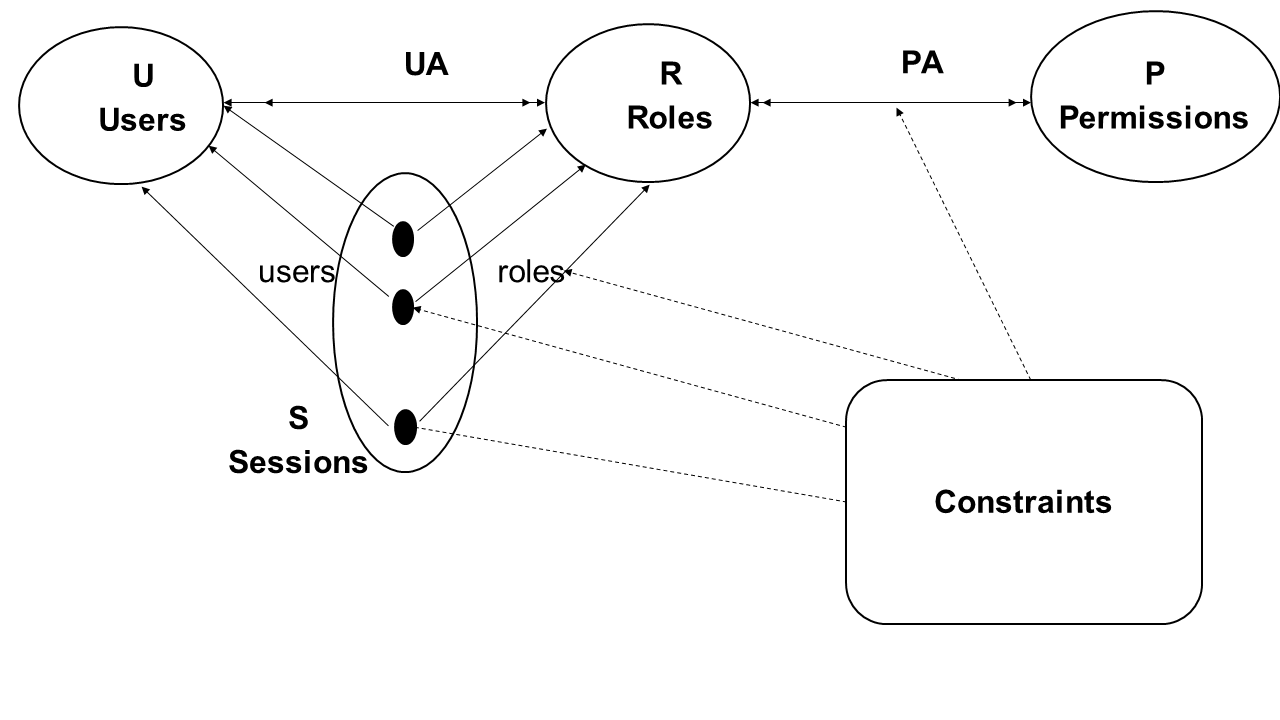
\includegraphics[scale=0.26]{modelConstraints.png}
\caption{RBAC Model Constraints.}
\label{fig:RBACPol}
\end{figure}

Mutual exclusiveness of roles is one of the most common constraints for an RBAC model.  Usually, it is defined as Separation of Duties (SoD), where the same user cannot be assigned to two conflicted roles at the same time~\cite{FeKu2009}.  For example, for two roles $R1$ and $R2$ belonging to mutually exclusive sets of roles, then if a user $U$ is assigned to $R1$, this implies that $U$ cannot be assigned to $R2$, and vice versa.  This is expressed formally as the code appearing after the table.\ref{tab:elements}.
  
 
\begin{align*} 
If&  (U \times R1) \in UA \Rightarrow  (U \times R2) \notin UA ;     and \\
If&  (U \times R2) \in UA \Rightarrow (U \times R1) \notin UA
\end{align*}    


Cardinality constraints define the maximum number of users that can be assigned to a particular role.  Likewise, cardinality constraints can be used to specify the number of roles that can be related to a particular user.  In addition to that, they can be applied to Permission Assignment (PA) for the purpose of restricting the number of permissions that a particular role should be assigned to~\cite{SDAG2008}.





\section{The EMS System and its Entities}\label{sec:entities} 

The Electronic Marking System (EMS) allows students, teachers, headmasters and guardians to access students’ marks of their units.  Each user is able to benefit from the system according to the powers/authorizations given to him/her.  For example, students can electronically submit papers (reports) for a particular unit to be marked by the unit's teacher.  Teachers, on the other hand, have the right to establish, edit and delete marks of their students.  In addition, headmasters and guardians can also access the system for the purpose of viewing marks and signing final reports.  

\begin{figure}[bht]
\centering
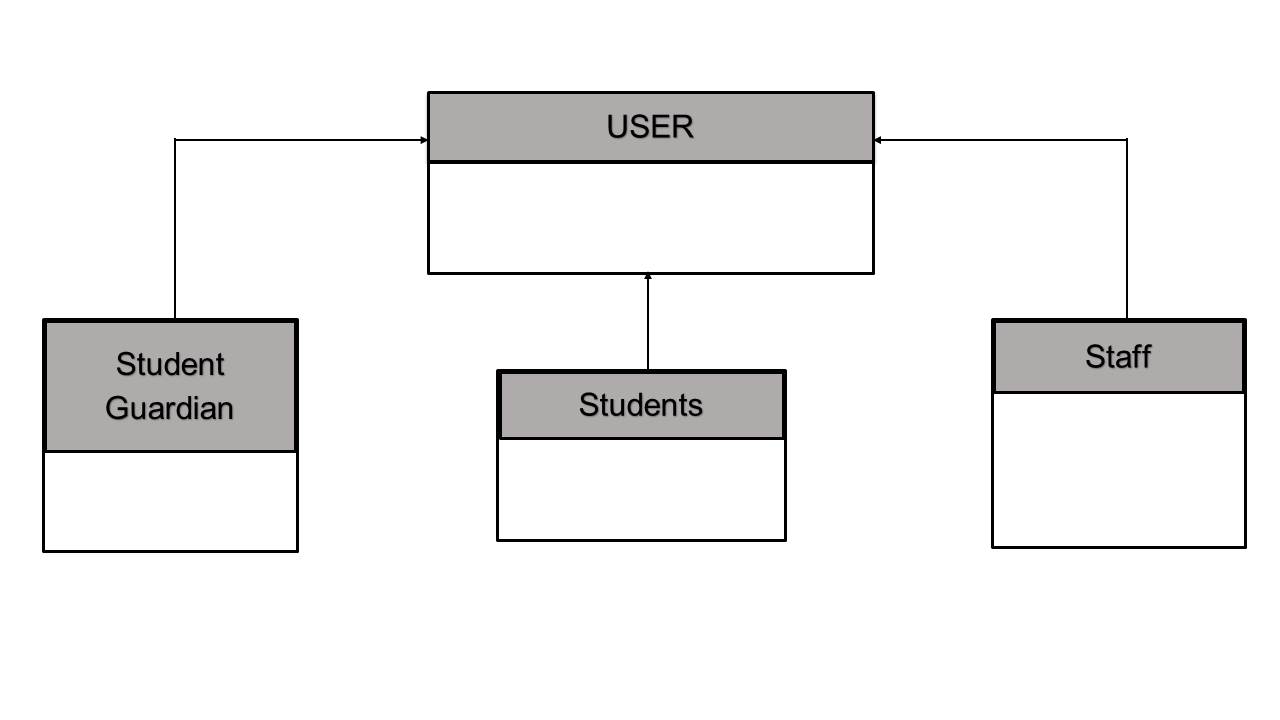
\includegraphics[scale=0.26]{EMSEntities.png}
\caption{Entities of the EMS's users.}
\label{fig:RBACPol}
\end{figure}

Generally, the EMS system can be accessed by different users: the system admin (who controls and manages the different entities and resources of the system), students, teachers, headmasters and guardians.  Hence, users can be classified into three main entities (tables): staff, students, and guardians, where staff entity represents teachers and headmasters as well as the system admin.
The other entities of the system as well as the relationships between those are briefly demonstrated in Table\ref{tab:otherentities} and Table\ref{tab:relations},respectively, in the following page.

\begin{table*}[bth]
\centering
\caption{Entities of the EMS System.}
\small
\rowcolors{0}{}{lightblue}
\begin{tabular}{p{0.8 in} p{6 in}} \hline 
\hline
Code & Description\\\hline\hline

UNIT& to represent all units taught at secondary schools. \\ 
SUBMISSION& to store submitted reports by students. \\ 
FINAL\_REPORT& which contains final reports for all students. \\ 
MARK& its contents are natural numbers, which represent students’ marks. \\ 
ROLES& this entity is set up for the purpose of applying RBAC model.  Hence, it represents the different roles in the EMS system (i.e. admin, teacher, student, etc.).\\ \hline\hline
\end{tabular}
\label{tab:otherentities}
\end{table*}




\begin{table*}[bth]
\centering
\caption{Relations between the EMS entities.}
\small
\rowcolors{0}{}{lightblue}
\begin{tabular}{p{0.9 in} p{5.9 in}} \hline 
\hline
Code & Description\\\hline\hline

studies &   represents a relation between a student and a unit; where each student studies more than one unit; and that unit can be registered for many students. \\

taughtBy &  a relation between a unit and a teacher; where each unit must be taught by at least one teacher; and that teacher can be registered to more than one unit.\\

hisGuardian &  a relation between a student and a guardian.  A student can have more than one guardian in order to facilitate the process of following up the student’s level.  In addition, the guardian can be registered for more than one student\\

submits &   a relation between a student and a submission; where any student can submit any number of reports (depending on the unit and the academic level that a student is studying at); however, any report cannot represent a submission for more than one student.\\

reportFor &  a relation between a submitted report and a unit.  Therefore, all submitted reports are for particular units, and each unit may have more than one report. \\

submissionMark &  a relation between a submitted report and a mark (which is a natural number).  However, it is not possible for a report to be mapped into two different marks (axiomatic!), but we can find that a given mark represents the grade of more than one report.\\

InClassMark &  a relation between a unit and a mark (i.e. natural number) to specify a student’s mark for his/her participations and activities inside the class during the year. \\

examMark &  a relation between a unit and a mark to specify the student’s mark/s (depending on how many exams for that unit).\\ 

studentReport &  a relation between a student and a final report; where each student must have a final report for each unit, which shows his/her final mark.  However, it is not reasonable to assign two final reports to the same student.\\

hasTheRole & maps a user into a set of roles (e.g. student, teacher, headmaster or student guardian); where each user would be linked to only one role (unless there were some circumstances made otherwise, e.g. in case of absence of the school manager, any teacher can be assigned to play the role of headmaster; and this assignment falls under the responsibility of the system’s admin).

\\ \hline\hline
\end{tabular}
\label{tab:relations}
\end{table*}










\section{Application of RBAC to the EMS}\label{sec:application} 

In order to apply an RBAC security policy to the EMS system, we need to define the different components of RBAC models (i.e. $RBAC_0$, $RBAC_1$ and $RBAC_2$).  For $RBAC_0$, it is essential to specify the sets of USERS, ROLES, and PERMISSIONS.

\subsection{RBAC0- Basic model}
Since the system has three main types of users (i.e. staff, students, students’guardains), each user represents an element in the USER set (U).  Regarding ROLES (R), there are six basic roles, which describe the main functionality for users in the Electronic Marking System (EMS).  These roles would be stored into the ROLES entity of the database.  Therefore, contents of this entity can be defined as follows:

\begin{align*}
ROLES = \{admin, student, teacher, headteacher, \\headmaster, student\_guardian\}
\end{align*}


Permissions (P) are pairs of (operations, objects) in which users are allowed to perform.  For example, a student wants to store a report $(operation)$ into SUBMISSION table $(object)$ in order for the report to be considered “submitted”.  This process means that the student is permitted to add a submission.  The EMS system allows each type of users to perform only specific permissions. 

\begin{figure}[bht]
\centering
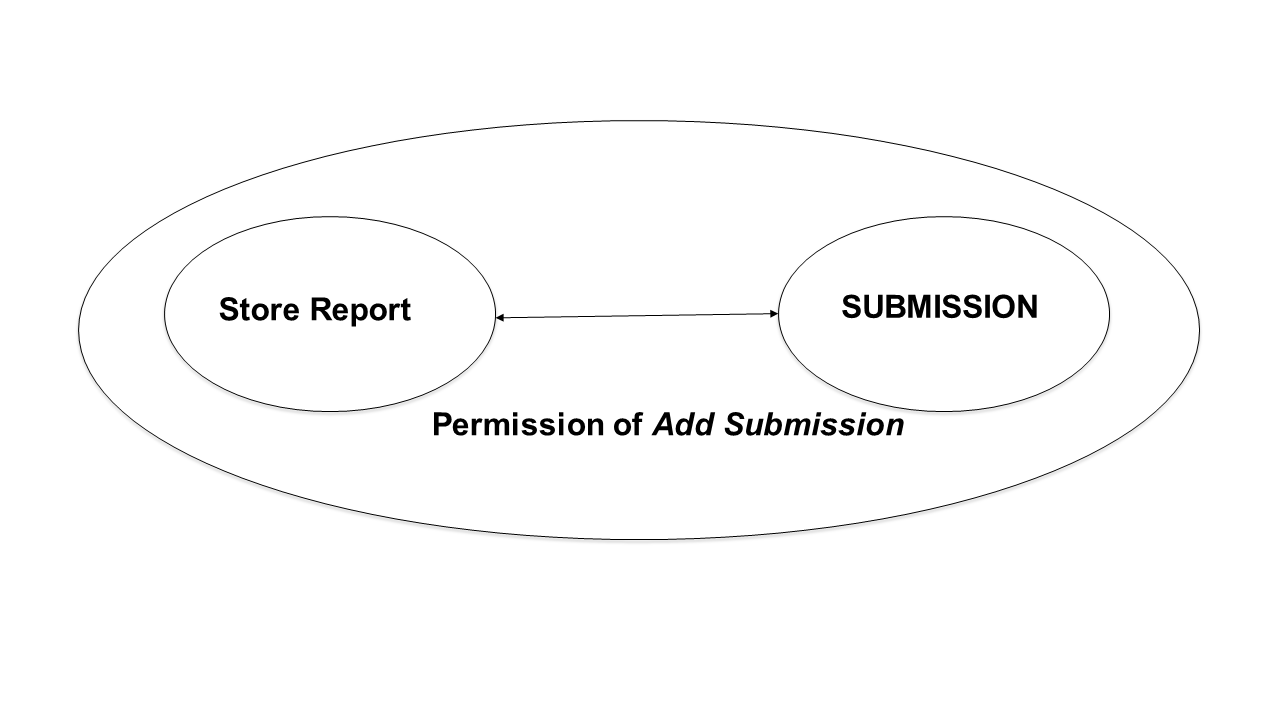
\includegraphics[scale=0.26]{addsubmission.png}
\caption{"Add Submission" permission for students.}
\label{fig:permstud}
\end{figure}

\subsection{User Assignment (UA) and Permission Assignment (PA)}
User Assignment (UA) is a many-to-many relationship between the system’s users U and the roles R.  For example, students take the role $student$, while teachers are assigned to role $teacher$.  In some cases, it is possible to assign a user to two different roles if a given situation requires that.  For instance, in case of absence of a headmaster, any teacher can be authorized to perform the headmaster permissions, and that would be done through giving the role $headmaster$ to the teacher, in addition to his/her own role.

Permission Assignment (PA) is also a many-to-many relationships, in which roles are mapped into permissions (functions).  There are specific functions for each role, where can only be performed by user(s) who is/are assigned to those roles.  The following diagram shows an example of Admin assignment:

\begin{figure}[bht]
\centering
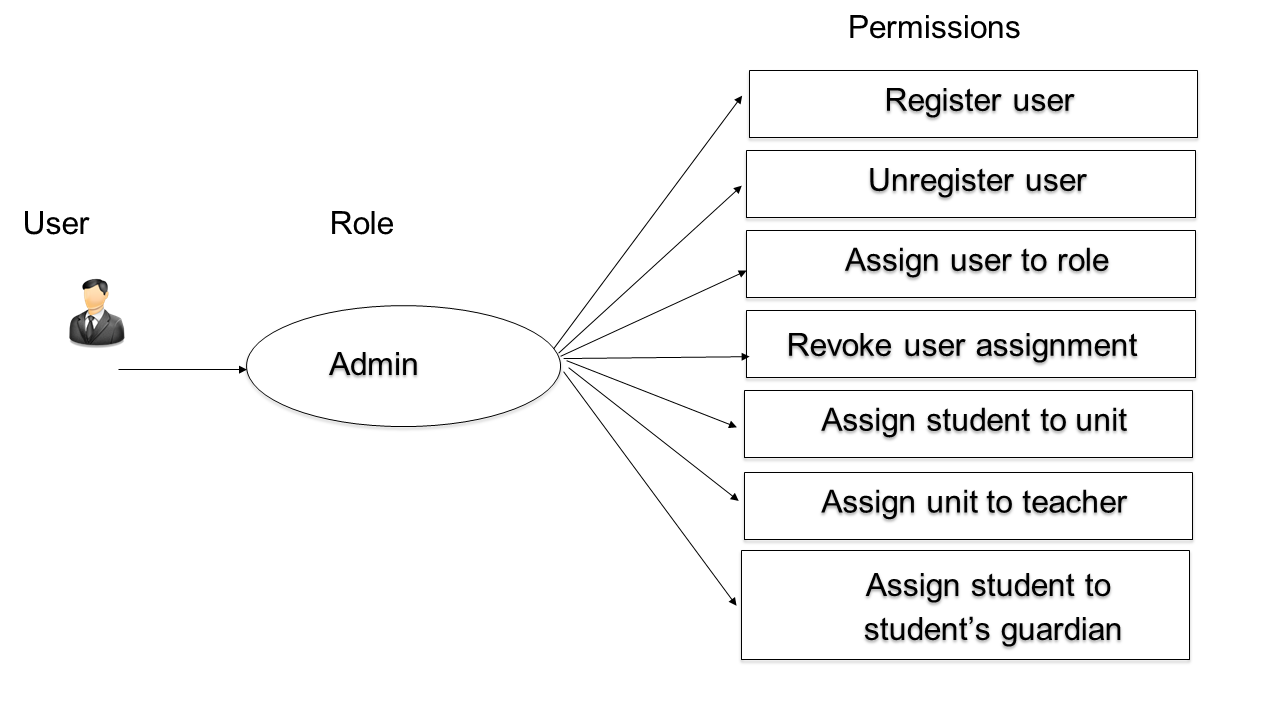
\includegraphics[scale=0.26]{addAdmin.png}
\caption{"Admin" role in the EMS System.}
\label{fig:permstud}
\end{figure}


\subsection{RBAC1- Role Hierarchy (RH)}

In the EMS system, there is only one instance of role hierarchy.  Head teachers are, in fact, teachers, although they have special tasks for organizing and monitoring roles assigned to teachers, such as reviewing records.  When a head teacher is assigned to role $headteacher$, this means that the head teacher is allowed to perform functions of the headteacher role, and inherit permissions from the role $teacher$.

\subsection{RBAC2- Constraints}

For the EMS system, there are two types of constraints that can be defined: cardinality constraints and mutual exclusiveness of roles.  Usually, cardinality constraints represent the number of users who should be assigned to a particular role.  In our system, it doesn’t matter how many students to be assigned to $student$ role, or how many teachers to be mapped into $teacher$ role, as that depends on the number of students and teachers inside a certain school.  However, there must be only one user who should take the role $headmaster$.  Thus, the cardinality constraint for role $headmaster$ is expressed as:

\begin{flalign*}
UA \subseteq U \times R\ \text{where}\ \\ 
\mathbf{card}(U (school manager)) \times \mathbf{card}(R(headmaster)) = 1
\end{flalign*}


Mutual exclusiveness of roles (Separation of Duties) define the conflicted sets of roles, which must not be related to the same user/s.  For example, if there are two roles $R1$ and $R2$ belonging to two conflicted sets of roles $S1$ and $S2$, respectively, then: If a user $U$ has been assigned to a role in $S1$, this implies that $U$ is not assigned to any role in $S2$, and vice versa.  

In the Electronic Marking System (EMS), there are two conflicted classes (sets) of roles:

\begin{flalign*}
SoD1 &= \{teacher, headteacher, headmaster\}, and \\
SoD2 &= \{student, student\_guardian\}
\end{flalign*} \\


\section{Modeling the RBAC Policy Using the B Language}\label{sec:modeling} 

     Analyzing RBAC models using a formal method, such as the B method or Event-B may assist system developers to obtain a correct and consistent specification.  By knowing RBAC constraints, formal specifications can play a significant role to examine security policies, and determine whether a particular system is secure at every point of time.
The B method is one of the abstract formal languages that uses a special language named “Abstract Machine Notation (AMN)”.  The idea is to use mathematical notations (relying on mathematical logic and set theory) to formalize specifications for the purpose of formally verifying correctness and consistency of a specification.

\subsection{Modeling the Basic RBAC Components}

To formalize the basic RBAC elements, it is essential to define the sets of USER and ROLES as well as UA and PA assignments.  In the EMS system, USER set contains subsets of students, guardians and staff.  The latter itself contains subsets of teachers and headmasters.  Therefore, these subsets must be declared as variables in the AMN: 

staff, students, studentGuarian, teachers, manager

Now, we can declare, within INVARIANT clause, that each of those variables is a subset of USER set, and some are also subsets of staff subset, provided that no element of each subset can be found into two different subsets.  For example, if a student has been registered into students subset, then that student cannot be found as a member of staff subset (i.e. students ∩ staff = { }).  This can be expressed using the B specification as follows:

students ⊆ USER  ∧
staff ⊆ USER  ∧
students ∩ staff = { }  ∧
studentGuardian ⊆ USER   ∧
studentGuardian ∩ students = { }   ∧
studentGuardian ∩ staff = { }   ∧
manager ⊆ staff   ∧
teachers ⊆ staff   ∧
manager ∩ teachers = { }

To model the User Assignment (UA), which assigns each user to a particular role, we need to define a relation between USER set and ROLES set.  This relation is, in fact, a set of elements, where each element is a pair of user and role.  For example, if a user u has been assigned to a role r, then there is an element for the relation can be defined as: {(u, r}}.

Since elements of the relation between USER and ROLES are subject to change (i.e. assigning new users to roles, or revoking existing assignments), we represent this relation as a variable, and we give it the name: hasTheRole.  The declaration of that within the INVARIANT clause would be as: 

hasTheRole ∈ USER ↔ ROLES

To model the Permissions Assignments (PA), we do not need to define a new set for permissions, or a direct relation (as in the UA assignment) between ROLES and those permissions.  Since any permission is actually a pair of operation and object, we will be specifying (within preconditions of each operation (function)) in the system, that this operation is only performed by users who have been given a particular role.

For example, users who can add a submission are only students.  Therefore, we say, as a precondition of the operation, that “who has the role of ‘student’, can perform this operation”.  This is expressed by the B specification as in Figure 8:


\subsection{Modeling the RBAC Constraints}

     We begin with mutual exclusiveness of roles  (Separation of Duties).  As has been mentioned earlier, there are two conflicted sets of roles in the EMS system.  Since roles are previously known and defined for the system, the two conflicted sets of roles should be initialized within the INITIALIZATION clause as:

$sod1 = {teacher, headteacher, headmaster}$,
$sod2 = {student, student_guardian}$

     Each of sod1 and sod2 is a subset of ROLES set, and the intersection between them is equal to an empty set.  Therefore, this must be declared within INVARIANT clause:
sod1 ⊆ ROLES  ∧
sod2 ⊆ ROLES  ∧
sod1 ∩ sod2 = { }
     Now, we can formulate the condition of Separation of Duties (SoD) using the B specification, as follows:

∀(u, role1, role2). (u ∈ USER  ∧  role1 ∈ sod1  ∧  role2 ∈ sod2  ∧  
        role1  ∈   hasTheRole[{u}]         ⇒  not (role2 ∈ hasTheRole[{u}] )  ∧

  ∀(u, role1, role2). (u ∈ USER  ∧  role1 ∈ sod1  ∧  role2 ∈ sod2  ∧  
        role2 ∈   hasTheRole[{u}]       ⇒  not (role1 ∈ hasTheRole[{u}] )  

     The above two predicates mean, respectively, that for every user u and two given roles role1 and role2, where u ∈ USER and role1 ∈ sod1 and role2 ∈ sod2 and that role1 belongs to the set of roles given to the user u, then the role2 must not belong to the roles of the user u.  Likewise, for every user u and two given roles role1 and role2, where u ∈ USER and role1 ∈ sod1 and role2 ∈ sod2 and that role2  belongs to the set of roles given to the user u, then the role1 must not belong to the roles of the user u
     The second type of constraints is cardinality constraints.  In the EMS system, the number of users who will be assigned to headmaster role must not be greater than 1.  Hence, the cardinality of users who have the role headmaster must be less than or equal to 1.  This is expressed as: 

∀(headmaster). (headmaster ∈ sod1  ⇒ 
                            card(hasTheRole-1[{headmaster}]  ≤ 1 )  

\subsection{Modeling the Role Hierarchy (RH)}
     Head teachers have their own permissions, such as reviewing records.  However, they still teachers, and, therefore, can perform operations that are given to teachers.  We need to formulate a predicate that satisfies the concept of inheritance, where head teachers can inherit permissions from teacher role.  In the B specification, this is expressed as:

∀(u, headteacher). (headteacher  ∈ sod1  ∧  u ↦ headteacher   ∈ hasTheRole
⇒  headteacher  ∈ hasTheRole[{u}]   ∧  teacher  ∈ hasTheRole[{u}] )

    Which means that for every user u and headteacher role, where headteacher ∈ sod1 and that user has been assigned to the role headteacher, then the user u would become have the role teacher in addition to the role headteacher.


\section{The Efficiency of the Proposed Solution} 

By looking at the work mechanism of RBAC models, we may find that strength of RBAC policies lies in the fact that users are not directly connected to the implementation of operations. Rather, there should be some roles to be previously linked to specific permissions, and users are being assigned to those roles according to requirements of a system. 

The work on applying the concept of UA and PA is the critical point for ensuring that users are performing correctly the operations allocated for them.  User assignments and permission assignments can be defined as links between three different sets (i.e. users, roles and permissions).  In our specification, UA has been clearly declared as:
          

\begin{align*}
hasTheRole \in USER \leftrightarrow ROLES
\end{align*}


However, there were no declaration for PA, where roles need to be mapped into permissions.  Instead, we adopted the strategy of restricting the performance of operations by certain users, through stating some checking predicates within the preconditions of each operation in the system.  This is precisely what is mostly applied in some programming languages for development of web applications (e.g. Java). When roles of the system are defined (usually via a realm), the link between those roles and permissions is done within the structure of the functionality itself.  

For instance, in the EMS system, the only users who can add a submission mark are teachers (who are assigned to the role $teacher$).  Hence, we make the link between this role and the function of adding a submission mark through the following statement (as a precondition): 


\begin{align*}
hasTheRole[\{t\}] = \{teacher\} 
\end{align*}



This predicate means that if the user $t$ has the role of $teacher$, then he will be able (if also satisfying the other preconditions- see algorithm 2) to perform the operation.  The following algorithm shows the B code for the operation of adding a submission mark.

 \begin{algorithm}                      % enter the algorithm environment
 	\caption{Assigning "add a submission mark" permission to "teacher" role}          % give the algorithm a caption
 	\label{alg1}                          
 	%\begin{algorithmic}  
 	
 	
 	PRE \\
 	
 	\quad ${\bf hasTheRole[\{s\}] = \{student\}} \wedge$\\
 	
 	\quad $report \in SUBMISSION \wedge$ \\
 	
 	\quad $report \notin reports \wedge$ \\
 	
 	\quad $u \in studies [\{s\}] \wedge$ \\
 	
 	\quad $card(submit[\{s\}] \cap reportFor[\{u\}]$ \\
 	
 	\quad $< maxSubmissions$
 	
 	
 	
 	THEN \\ 
 	
 	\quad $report \gets reports \cup \{report\} \mid\mid \\$
 	
 	\quad $submits \gets submits \cup \{s \mapsto report\} \mid\mid \\$
 	
 	\quad $reportFor \gets reportFpr \cup \{report \mapsto u\}$
 	
 	
 	END
 	%\end{algorithmic} 
 \end{algorithm} 


\section{Formal Verification}\label{sec:verification} 

Perhaps the most important aspect in using formal methods in software development is that specifications can be analyzed and verified using mathematical techniques and tools.  There are two approaches for formal verification: model checking and theorem proving (e.g. proof obligations).

\subsection{Model Checking (the ProB tool)}
 
Model checking is an automated approach that used to verify correctness and consistency of a model.  The ProB tool is one of the B machines-supported tools that test automatically the consistency of the B specification.  The main idea of model checking is that all machine nodes (states) are visited to examine whether there exist any potential bugs~\cite{MMFA2012}.

The $ProB$ tool showed that our RBAC specification is correct regarding the system states (nodes).  There was no violation with the system properties and invariant when it comes to the performance of operations.

\subsection{Theorem Proving (Proof Obligations)}
The main purpose of theorem proving is to construct a mathematical proof for a mathematical statement to be true~\cite{Bou2012}.  Since formal proofs do not use natural languages, they are expressed in a symbolic language, usually called a proof language. 
For abstract machines to be correct and consistent, there are many proof obligations that need to be proven.  Theses proof obligations are for the four main clauses of an abstract machine: PROPERTIES, INVARIANT, INITIALISATION and OPERATIONS, where there is a separate proof obligation for each operation in the machine~\cite{MMFA2012}. 


Since our RBAC model does not have properties clause, proof obligations would be for the clauses of INVARIANT, INITIALISATION and OPERATIONS.  Proof obligation for invariant clause is expressed as:

\begin{align*}
Prp \Rightarrow  \exists \quad v. \quad I
\end{align*}

      Which means that under the assumption that $Prp$ (PROPERTIES clause, if found) is true, then: the invariant $I$ is satisfied by at least one of the machine variables $v$.
     To discharge this obligation, we need to show that there exist values for:
     
\begin{itemize}
\item \emph{sod1} and \emph{sod2}, which are subsets of \emph{ROLES}; where the intersection between them is an empty set.
\item	\emph{hasTheRole}, which is a relation between \emph{USER} and \emph{ROLES}; where:
\begin{itemize}
\item for any user and two conflicted roles, the concept of SoD is applied;
\item for any user has the role $headteacher$, the concept of Role Hierarchy is applied; and
\item cardinality of users who take the role $headmaster$ is less than or equal to 1. 
\end{itemize}
\item	\emph{staff, teachers, manager, students} and \emph{studentGuardian}, which are subsets of \emph{USER}; where:
\begin{itemize}
\item	teachers and manager are subsets of staff; and
\item	the intersection between any two subsets is an empty set.
\end{itemize}
\item \emph{hisGuardain}, which is a partial surjective function between $students$ and $studentGuardain$.

\end{itemize}

Perhaps the easiest way to demonstrate that is to apply the current values of variables in the INITIALISATION clause (i.e. all variables are equal to \{\}, except the sets of $sod1$ and $sod2$).  

      
      The proof obligation for INITIALIZATION takes the following predicate: 

\begin{align*}
Prp \Rightarrow[Init] I
\end{align*}



Which means that under the assumption that $Prp$ (PROPERTIES clause, if found) is true, then: the initialisation clause $Init$ must establish the invariant $I$.  To demonstrate this obligation, we apply the current values in the INITIALISATION clause to their corresponding variables in the INVARIANT clause.

For each operation in the machine, there must be a separate proof obligation.  Hence, there will be proof obligations for $assignUserToRole$ and $revokeUserAssignment$ operations.  The proof obligation of each operation takes the following predicate: 

\begin{align*}
I \wedge P \Rightarrow [S] I
\end{align*}



Which means that under the assumption that invariant $I$ is true and the preconditions $P$ of the operation is true as well, then: the statement of the operation $S$ (i.e. the body of the operation) must preserve the invariant $I$.


\section{Conclusion}\label{sec:conclusion} 

RBAC security policy is considered as one of the most effective security models to different critical systems, such as business systems.  Formal specification is now widely used to verify security constraints/properties of RBAC models in different ways and several languages.  This paper discussed the use of the B method to develop a consistent specification for the RBAC security policy of an Electronic Marking System (EMS).   There has been the use of two approaches for formal verification: model checking and proof obligations.  Model checking was represented by the application of proB tool, while proof obligations constructed a mathematical statement/proof for the RBAC model to be true.  Both mechanisms proved that our RBAC specification is correct and consistent regarding the implementation of the system operations.


%\section*{Acknowledgments}

%This work was supported by the BMBF within EC SPRIDE, the Hessian LOEWE excellence initiative within CASED, and a Fraunhofer Attract grant. 

%\bibliographystyle{abbrvnat}

\bibliographystyle{IEEEtranS}
\bibliography{RBACcontrolledSystem}


\end{document}

